\documentclass{article}
\usepackage[utf8]{inputenc}
\usepackage{hyperref}
\hypersetup{
colorlinks=true,
    linkcolor=black,
    filecolor=black,      
    urlcolor=blue,
    citecolor=black,
}
\usepackage[letterpaper, portrait, margin=1in]{geometry}
\usepackage{enumitem}
\usepackage{amsmath}
\usepackage{booktabs}
\usepackage{graphicx}
\usepackage{titlesec}
\usepackage[section]{placeins}

\titleformat{\section}
{\normalfont\Large\bfseries}{\thesection}{1em}{}[{\titlerule[0.8pt]}]
  
\title{Homework 4 \\ Economics 7103}
\author{Ana Mazmishvili}
\date{February 12}
  
\begin{document}
  
\maketitle

\section{Python}

\noindent 1. As we see from the figure \ref{fig:trend}, the treatment and control groups do not have perfect parallel trends, but the gap between them are still similar. Although the difference remains consistent over time until December 2017, a markedly sharp decrease in bycatch is observed right before treatment.

\begin{figure}[h]
    \centering
    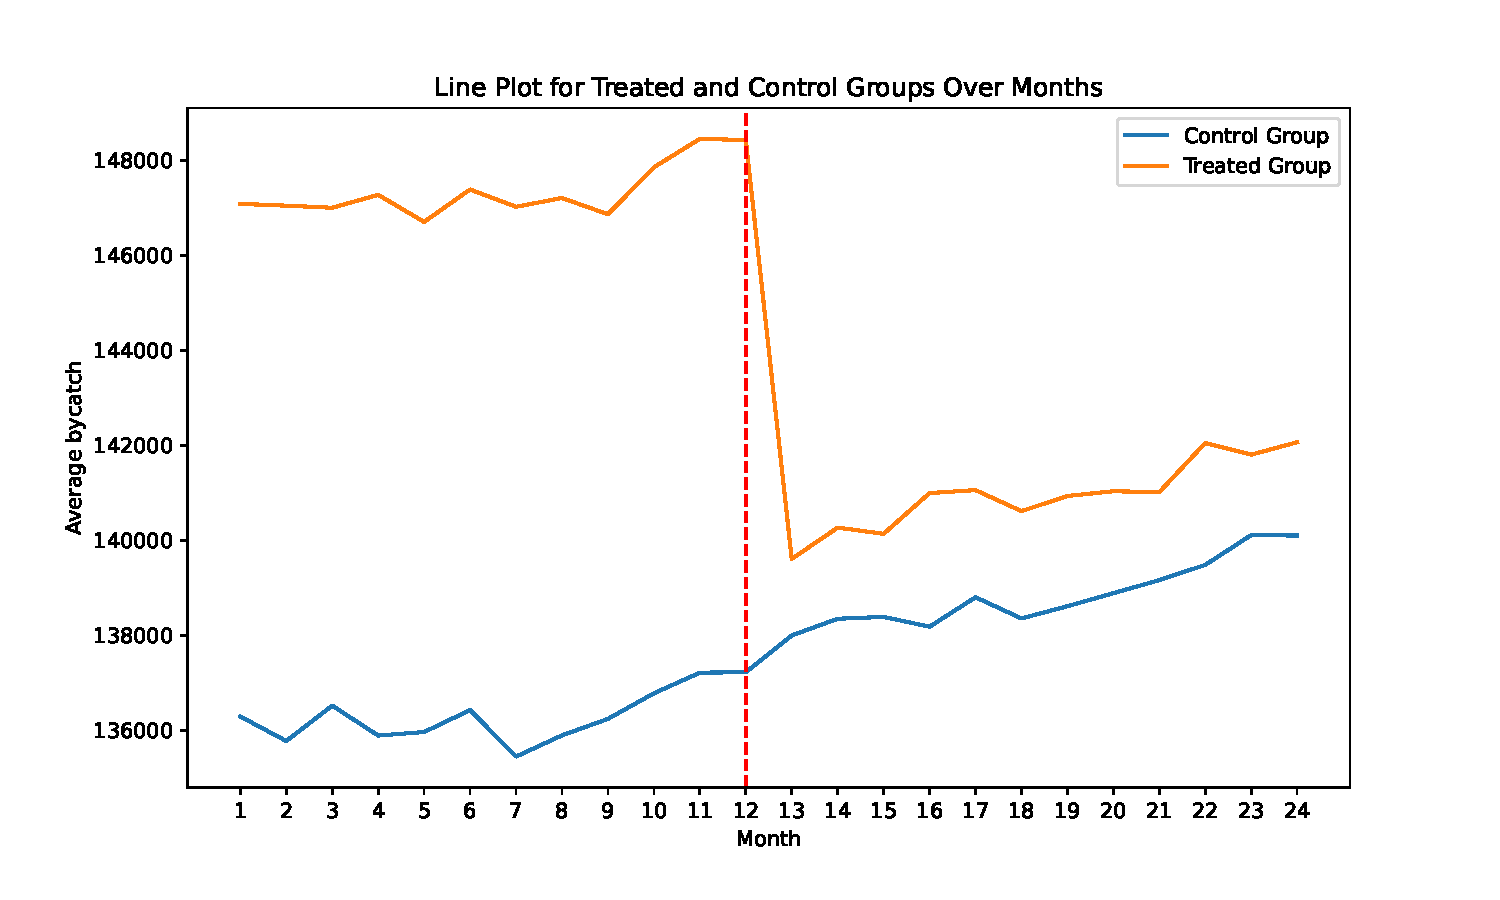
\includegraphics{homework 4/output/figure/trend1.pdf}
    \caption{ Bycatch by months before and after treatment. }
    \label{fig:trend}
\end{figure}

\FloatBarrier

\noindent 2. I manually estimated using Python the treatment effect of the program on bycatch using the sample analog of the population difference-in-differences for the treatment and control groups in December 2017 and January 2018. The results are presented in table \ref{tab:DID1}

\begin{table}[]
    \centering
    \begin{tabular}{rl}
\toprule
 & Sample analog of the population DID \\
\midrule
$\E[Y_{igt}|g(i) = treat, t=Dec2017]=$ & 148430.64 \\
$\E[Y_{igt}|g(i) = treat, t=Jan2018]=$ & 139612.51 \\
$\E[Y_{igt}|g(i) = control, t=Dec2017]=$ & 137228.60 \\
$\E[Y_{igt}|g(i) = control, t=Jan2018]=$ & 138001.81 \\
$\midrule DID = $ & -9591.35 \\
\bottomrule
\end{tabular}

    \caption{The sample analog of the population difference-in-differences}
    \label{tab:DID1}
\end{table}

\FloatBarrier

\noindent 3. Each method produces quite similar results that probably only differ in rounding error:


\noindent 4. See table .  If randomization worked, the simple difference-in-means is an unbiased estimate of the treatment effect.

\section{Stata}

\noindent \textbf{1.a.} I generated firm and month indicator variables and included all of them in the regression. Stata dropped two firm indicator variables and one month indicator variable. The DID estimator is presented in the first column of the Table \ref{tab:OLS}. \\

\noindent \textbf{1.b.} After demeaning at the firm level, "firmsize", "firm" and "month" dummy variables were eliminated. The DID estimator is presented in the second column of the Table \ref{tab:OLS}. \\

\noindent \textbf{1.c} The table \ref{tab:OLS} summarizes the results of estimating models in part (a) and (b). In the first model, the results indicate that treated firms decreased bycatch by 8,085 pounds. In the demeaned OLS regression results, treated firms, on average, reduced bycatch by 8,149 pounds relative to the control group after accounting for group-specific time trends.

\begin{table}[]
    \centering
    \begin{tabular}{l*{3}{c}}
\hline\hline
                    &\multicolumn{1}{c}{(a)}&\multicolumn{1}{c}{(b)}&\multicolumn{1}{c}{(c)}\\
\hline
Tretment Effect Estimates&    -8085.14&    -8085.14&    -8149.06\\
                    &   (2619.21)&   (2563.92)&   (2489.02)\\
\hline
Method              &OLS with Firm & Month FE&Demeaned OLS with Month FE&Demeaned OLS without Month FE\\
Observations        &        1200&        1200&        1200\\
\hline\hline
\end{tabular}

    \caption{Estimating the DID estimators using OLS regression}
    \label{tab:OLS}
\end{table}

\end{document}